%%%%%%%%%%%%%%%%%%%%%%%%%%%%%%%%%%%%%%%%%%%%%%%%%%%%%%%%%%%%%%%%%%%%%%%%%%%%%%%%
% > Лабораторная работа 6: Критические угловые скорости гибкого вала.
% > Баталов Семен, Антонова Мария, Клюшин Максим, Хайретдинова Диана.
% > 2021 год.
%%%%%%%%%%%%%%%%%%%%%%%%%%%%%%%%%%%%%%%%%%%%%%%%%%%%%%%%%%%%%%%%%%%%%%%%%%%%%%%%

\documentclass[12pt, a4paper]{article}
\usepackage[left=2cm, right=2cm, top=2.5cm, bottom=2.5cm, nohead, 
footskip=1cm]{geometry}
\usepackage{graphicx}
\graphicspath{{./Pictures/}}
\usepackage[utf8]{inputenc}
\usepackage[english, russian]{babel}
\usepackage{indentfirst}
\usepackage{array}
\usepackage{longtable}
\usepackage{misccorr}
\usepackage{setspace, amsmath}
\usepackage{multirow}

\begin{document}
    
    \newcolumntype{M}[1]{>{\centering\arraybackslash}m{#1}}
    \renewcommand{\arraystretch}{1.4}
    
    \begin{center}
        \large{Санкт-Петербургский государственный университет} \\
        \large{Saint-Petersburg State University}\\
        \hfill \break
        \hfill \break
        \hfill \break
        \hfill \break
        \hfill \break
        \hfill \break
        \hfill \break
        \large{Кафедра теоретической и прикладной механики} \\
        \hfill \break
        \hfill \break
        \large{\textbf{ОТЧЕТ}} \\
        \large{\textbf{По лабораторной работе 6}} \\
        \large{<<Критические угловые скорости гибкого вала>>} \\
        \hfill \break
        \hfill \break
        \hfill \break
        \large{По дисциплине} \\
        \large{<<Лабораторный практикум по теоретической механике>>} \\
    \end{center}
    
    \hfill \break
    \hfill \break
    \hfill \break
    \hfill \break
    \hfill \break
    \hfill \break
    
    \begin{flushright} 
        \large{Выполнили:} \\
        \hfill \break
        \large{Баталов С. А.} \\
        \large{Антонова М. } \\
        \large{Клюшин М.} \\
        \large{Хайретдинова Д.} \\
    \end{flushright}
    
    \hfill \break
    \hfill \break
    \hfill \break
    \hfill \break
    
    \begin{center} 
        \large{Санкт-Петербург} \\
        \large{2021} \\
    \end{center}
    
    \thispagestyle{empty}
    \newpage
    
    \section{Описание установки}
    
    В данной работе рассматривается явление потери устойчивости прямолинейной формы вращающегося вала. Целью работы является экспериментальное определение первых двух критических угловых скоростей, наблюдение соответствующих форм потери устойчивости и сравнение полученных результатов с теоретическими.
    
    \begin{figure} [h]
        \centering
        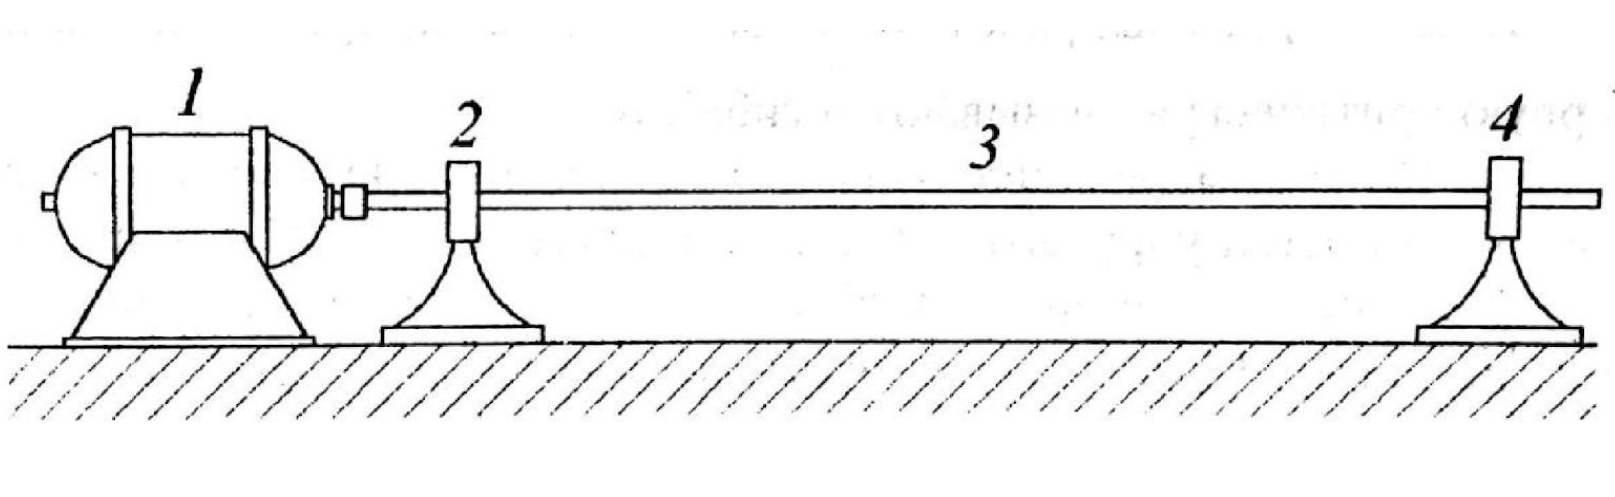
\includegraphics [width = 12cm] {Lab_6_1.png}
        \caption{\centering Схема лабораторной установки.}
        \label{im1}
    \end{figure}
    
    На рис.~\ref{im1} изображена схема лабораторной установки. Основной частью установки является гибкий деревянный вал \textit{3}, установленный на станине в двух сферических подшипниках \textit{2} и \textit{4}. Вал может скользить вдоль оси подшипника \textit{4}. Описанный способ крепления дает валу возможность вращаться не только в прямолинейном, но и в изогнутом состоянии. Вал \textit{3} связан с валом электродвигателя \textit{1}, находящегося на станине.
    
    \newpage
    
    \section{Параметры установки}
    
    В следующей таблице представлены параметры установки: плотность материала вала~--~$\rho$, модуль упругости материала вала~--~$E$, диаметр вала~--~$d$, длина вала~--~$l$.
    
    \begin{longtable}{ | M{2cm} | M{3cm} | M{3cm} | M{3cm} | M{3cm} |}
        \caption{\centering Результаты измерений параметров установки.}
        \label{tb1} \\
        \hline
        Номер & Величина & Значение & Погрешность & Размерность \\
        \hline
        1 & $d$ & 0,018 & 0,0001 & м \\
        2 & $l$ & 1,970 & 0,0005 & м \\
        \hline
        3 & $\rho$ & 667 & -- & $\text{кг} / \text{м}^{3}$ \\
        4 & $E$ & $1,38 \cdot 10^{10}$ & -- & Па \\
        \hline
    \end{longtable}
    
    \newpage
    
    \section{Теоретические исследования}
    
    \newpage
    
    \section{Результаты расчетов}
    
    \begin{longtable}{| M{2cm} | M{3cm} | M{3cm} | M{3cm} |}
        \caption{\centering Критические угловые скорости.}
        \label{tb2} \\
        \hline
        Номер & Величина & Значение & Размерность \\
        \hline
        1 & $\omega_{1}$ & 52,035 & $1 / \text{с}$ \\
        2 & $\omega_{2}$ & 208,140 & $1 / \text{с}$ \\
        \hline
    \end{longtable}
    
    \newpage
    
    \section{Результаты экспериментов}
    
    \begin{longtable}{| M{2cm} | M{3cm} | M{3cm} | M{3cm} | M{3cm} |}
        \caption{\centering Экспериментальные значения критических угловых скоростей.}
        \label{tb7} \\
        \hline
        \multirow{2}{*}{Номер} &
        \multirow{2}{*}{Величина} &
        \multicolumn{2}{M{6cm}|}{Значение} &
        \multirow{2}{*}{Размерность} \\
        \cline{3-4}
        & & Теория & Эксперимент & \\
        \hline
        1 & $\omega_{1}$ & 52,035 &  & $1 / \text{с}$ \\
        2 & $\omega_{2}$ & 208,140 &  & $1 / \text{с}$ \\
        \hline
    \end{longtable}
    
    \newpage
    
    \section{Выводы}
    
    
\end{document}